
\subsection{Voorpagina}\label{voorpagina}

\subsubsection{Grid}

De template van de website bestaat uit een grid, een soort geraamte. Het grid is opgebouwd uit verschillende regio's. In elke regio kunnen blokken geplaatst worden. In de paragraaf \emph{Felix}\seeone{felix} staat beschreven hoe en welke je blokken kunt toevoegen aan een regio. 

\bigskip

\begin{center}
	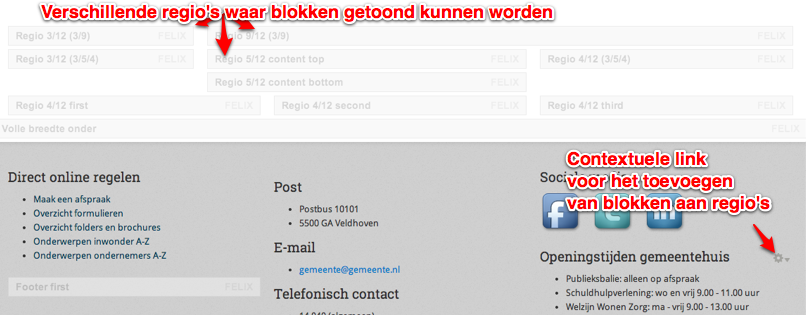
\includegraphics[width=\textwidth]{img/grid1.png}
\end{center}

\subsubsection{Blokken}

In het onderstaande afbeelding worden alle bestaande blokken op voorpagina in het kort toegelicht.

\bigskip

\begin{center}
	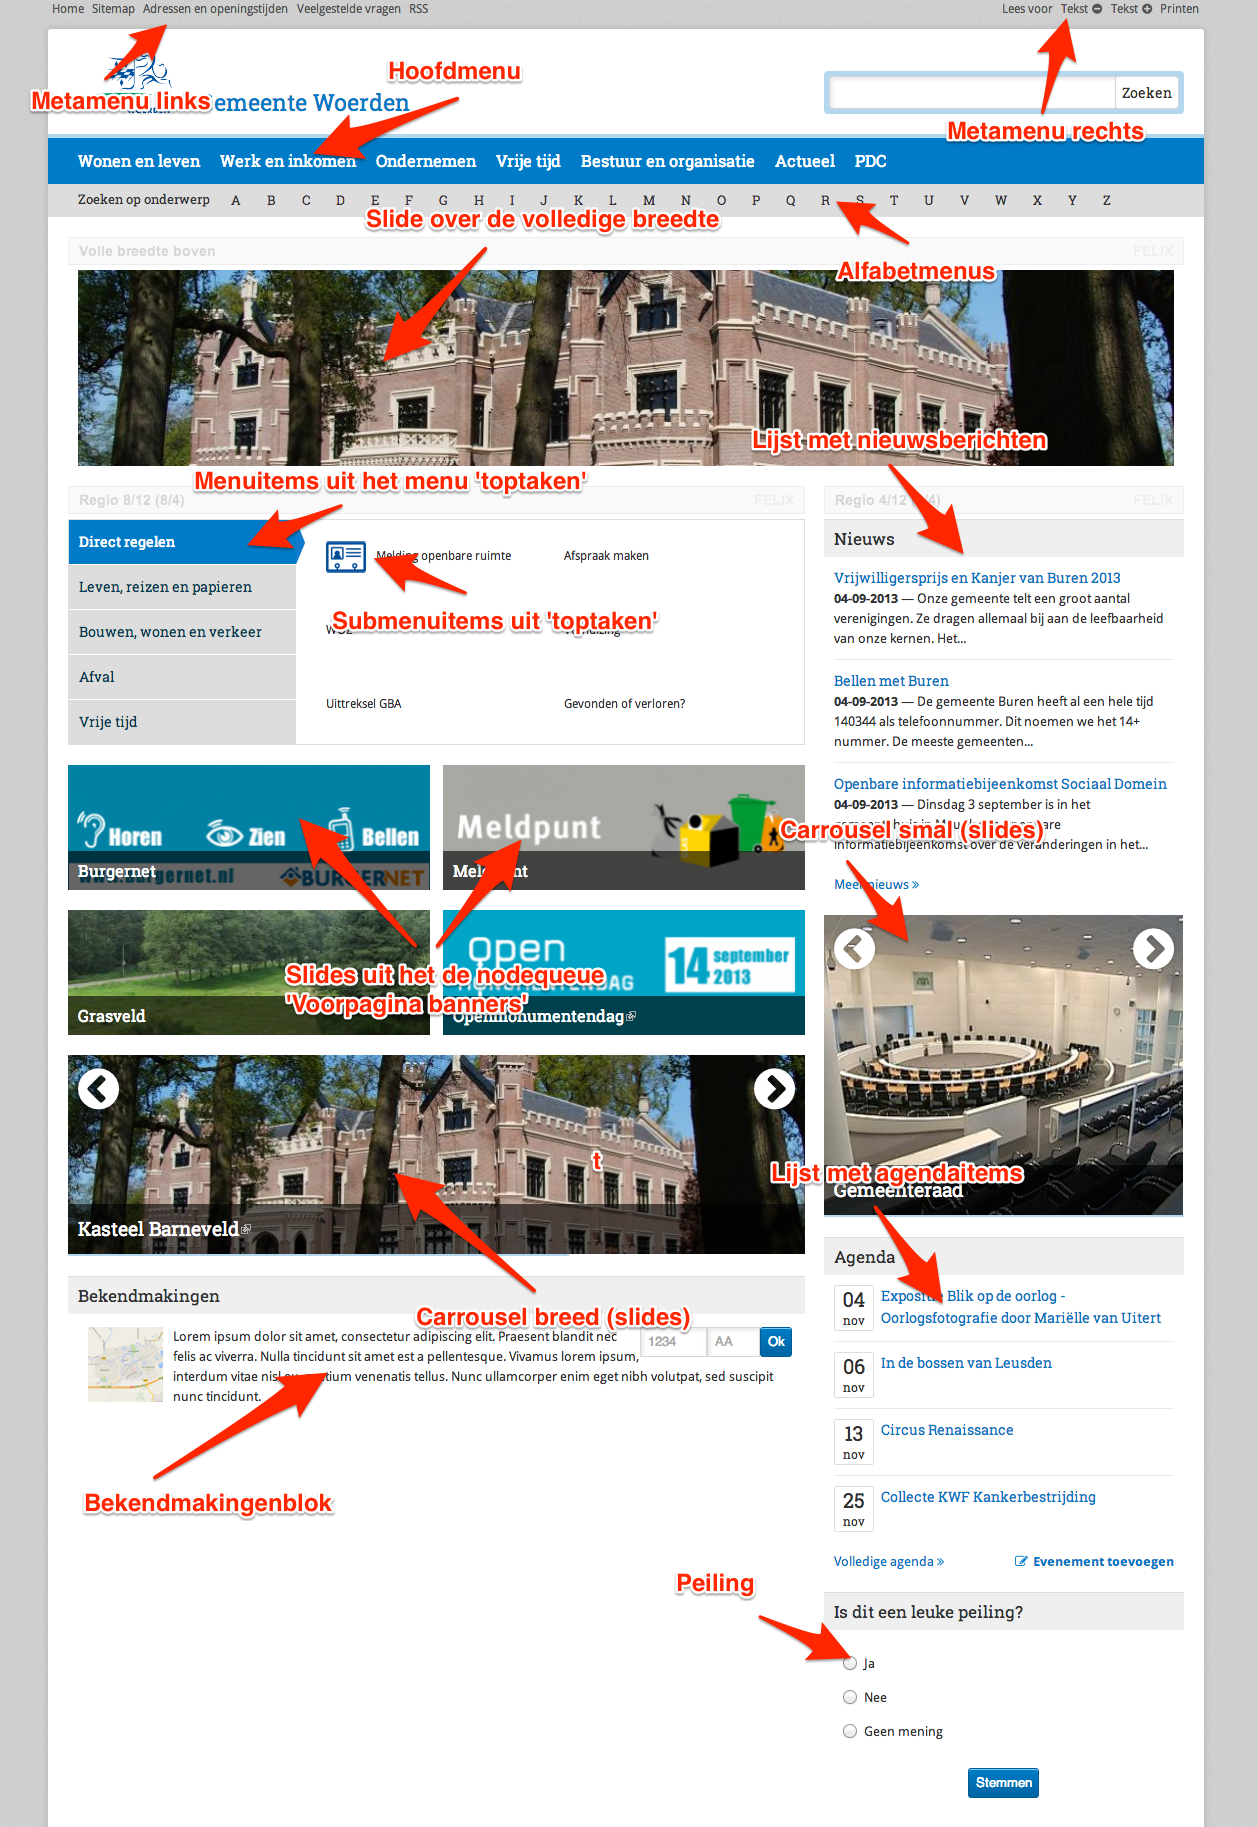
\includegraphics[width=\textwidth]{img/voorpagina.png}
\end{center}

\subsubsection{Footer}

In de onderstaande afbeelding worden de blokken, opgeleverd in het moedersjabloon, in de footer in het kort toegelicht. De footer bestaat uit 3 regio's waar blokken in gezet kunnen worden. Elke kolom is te vullen met Felix blokken bestaande uit items van het type Editorial. In de rechterkolom staan twee blokken: het eerste blok is het Dominion social blok. In paragraaf \emph{Social media}\seeone{socialmedia} staat beschreven hoe deze opties te beheren zijn. Daaronder staat nog een blok met redactionele content. De blokken die in deze regio's gezet worden, worden meegenomen door het hele domein.

\bigskip

\begin{center}
	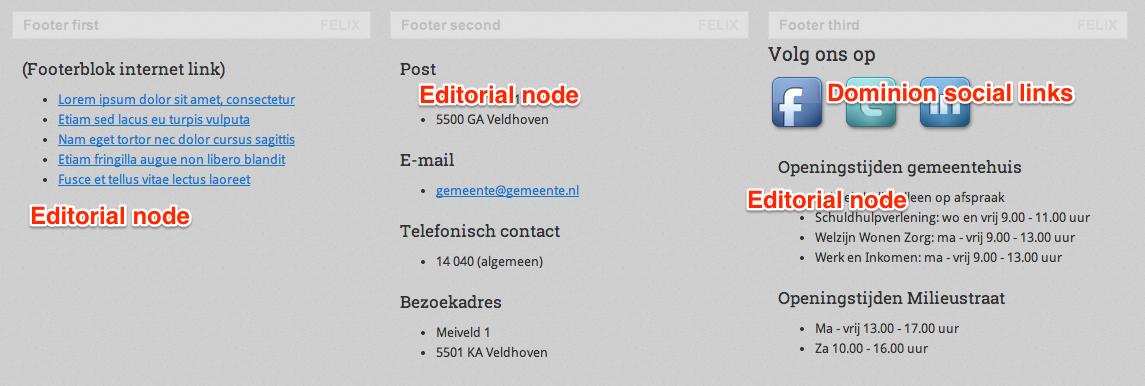
\includegraphics[width=\textwidth]{img/voorpagina3.png}
\end{center}